\documentclass[10pt,a4paper]{article}
\usepackage[utf8]{inputenc}
\usepackage[spanish,es-sloppy]{babel}
\usepackage{amsmath}
\usepackage{amsfonts}
\usepackage{amssymb}
\usepackage{graphicx}
\usepackage{tcolorbox}
\usepackage{here}
\usepackage{tikz}
\usepackage{animate}
\usepackage{url}
\usepackage{pgfplots}
\usepackage{cite}
\usepackage[left=1.8cm,right=1.8cm,top=1.5cm,bottom=1.5cm]{geometry}
\usepackage{verbments}

\newcommand{\mrm}{\mathrm}
%\definecolor{fondo1}{rgb}{0.9764, 0.9764, 0.9762}
%\definecolor{fondo2}{rgb}{0.1647, 0.4980, 0.7}
\definecolor{fondo1}{rgb}{0.88, 0.88, 0.88}
\definecolor{fondo2}{rgb}{0.15, 0.15, 0.5}
\author{Josue Huaroto Villavicencio - 20174070I\\Sección: E}
\title{6$^{\circ}$ Práctica de Cálculo por Elementos Finitos - MC516}
\begin{document}
\fvset{frame=bottomline, framerule=0.02cm,numbers=left, numbersep=8pt}
\plset{language=python,texcl=true,listingnamefont=\sffamily\bfseries\color{white},captionbgcolor=fondo2, bgcolor=fondo1,listingname=\textbf{Código}, captionfont=\sffamily\color{white},fontsize=\normalsize}
\tcbset{colframe=black!50!gray,colback=gray!20,colupper=black,fonttitle=\bfseries,nobeforeafter,center title}

\maketitle

\section{Ejecución del código}
Similar al código usado para las coordenadas y ángulos en una armadura plana, para la estructura del bastidor es necesario modificar la función de rigidez del elemento y la unión de estas matrices.
\begin{pyglist}[language=python,caption={Ensamble de la matriz de rigidez},style=pastie]
def ElementStiffness(l,angle,A,I):
    w = [A*np.cos(angle)**2+12*I*np.sin(angle)**2/(l*l),
         A*np.sin(angle)**2+12*I*np.cos(angle)**2/(l*l),
         (A-12*I/(l*l))*np.cos(angle)*np.sin(angle),
         6*I*np.sin(angle)/l,
         6*I*np.cos(angle)/l]
    aux = [[w[0],w[2],-w[3],-w[0],-w[2],-w[3]],
           [w[2],w[1],w[4],-w[2],-w[1],w[4]],
           [-w[3],w[4],4*I,w[3],-w[4],2*I],
           [-w[0],-w[2],w[3],w[0],w[2],w[3]],
           [-w[2],-w[1],-w[4],w[2],w[1],-w[4]],
           [-w[3],w[4],2*I,w[3],-w[4],4*I]]
    aux = np.array(aux)
    aux = aux*E/l
    return aux
    
def AssemblyStiffness(nStiffnessMatrix,k,i,j):
    for p in range(0,3):
        for m in range(0,3):
            nStiffnessMatrix[3*i+p][3*i+m] += k[p][m]
            nStiffnessMatrix[3*i+p][3*j+m] += k[p][3+m]
            nStiffnessMatrix[3*j+p][3*i+m] += k[p+3][m]
            nStiffnessMatrix[3*j+p][3*j+m] += k[p+3][3+m]
\end{pyglist}
Todos los demás elementos del código permanecen igual; ahora solo se necesita definir las condiciones del problema a resolver.
\begin{pyglist}[language=python,caption={Condiciones del problema},style=pastie]
NodesCondition = []
Nodes = 5
Nodes *= 3
NumberOfElement = 6
n = 12

Nodes = Nodes+3*(n-2)*NumberOfElement
NumberOfElement *= (n-1) 

h = 1500 #mm
E = 3.2e5 #MPA
K = []
A = (0.25*np.pi*(50)**2) #mm$^{2}$
I = (np.pi*50**4)/64 #mm${^4}$
L = []
P_A = 5000 #N
P_B = 4200 #N 
P_C = 2500 #N 
P_E = 3000 #N

PosNodes =  []
Elements = []

for i in range(0,n):
    PosNodes.append((i*h/(n-1),0))
for i in range(1,n):
    PosNodes.append((h,i*h/(n-1)))
for i in range(1,n):
    PosNodes.append((h-i*h/(n-1),h))
for i in range(1,n-1):
    PosNodes.append((i*h/(n-1),h-i*h/(n-1)))
for i in range(1,n):
    PosNodes.append((h+i*h/(n-1),h))
for i in range(1,n-1):
    PosNodes.append((2*h-i*h/(n-1),h-i*h/(n-1)))

for i in range(0,4*n-5):
    Elements.append((i,i+1))
Elements.append((4*n-5,n-1))
Elements.append((2*n-2,4*n-4))
for i in range(4*n-4,6*n-8):
    Elements.append((i,i+1))
Elements.append((6*n-8,n-1))

PosNodes = np.array(PosNodes)
Elements = np.array(Elements)
for i in range(0,NumberOfElement):
    L.append(DistNodes(PosNodes[Elements[i][0]],PosNodes[Elements[i][1]]))
L = np.array(L)

for i in range(0,NumberOfElement):
    K.append(ElementStiffness(L[i][0],L[i][1],A,I))

StiffnessMatrix = np.zeros((Nodes,Nodes))

U = np.zeros(Nodes).reshape(Nodes,1)
F = np.zeros(Nodes).reshape(Nodes,1)

Initialize(StiffnessMatrix,U,F)

#Node in UBoundary = Node*3+(x=0,y=1,theta=2)
UBoundaryCondition(U,0,3*0+0) #Nodo 0 en X
UBoundaryCondition(U,0,3*0+1) #Nodo 0 en Y
UBoundaryCondition(U,0,3*0+2) #Nodo 0 en theta
UBoundaryCondition(U,0,3*(3*n-3)+0) #Nodo 1 en X
UBoundaryCondition(U,0,3*(3*n-3)+1) #Nodo 1 en Y
UBoundaryCondition(U,0,3*(3*n-3)+2) #Nodo 1 en theta

FBoundaryCondition(F,-P_C,3*(n-1)+1) #Nodo 2 en Y
FBoundaryCondition(F,-P_E,3*(2*n-2)+1) #Nodo 3 en Y
FBoundaryCondition(F,-P_B,3*(5*n-6)+1) #Nodo 4 en Y
FBoundaryCondition(F,P_A,3*(5*n-6)+0) #Nodo 4 en X

U,F=Solve(StiffnessMatrix,U,F)
print("Stiffness Matrix:\n",StiffnessMatrix,'\n')
print("Displacements:\n",U,'\n')
print("\nForces:\n",F)
\end{pyglist}

\section{Resultados del problema}
Al finalizar la ejecución del solver, obtenemos la matriz de rigidez:
\begin{figure}[H]
    \centering
    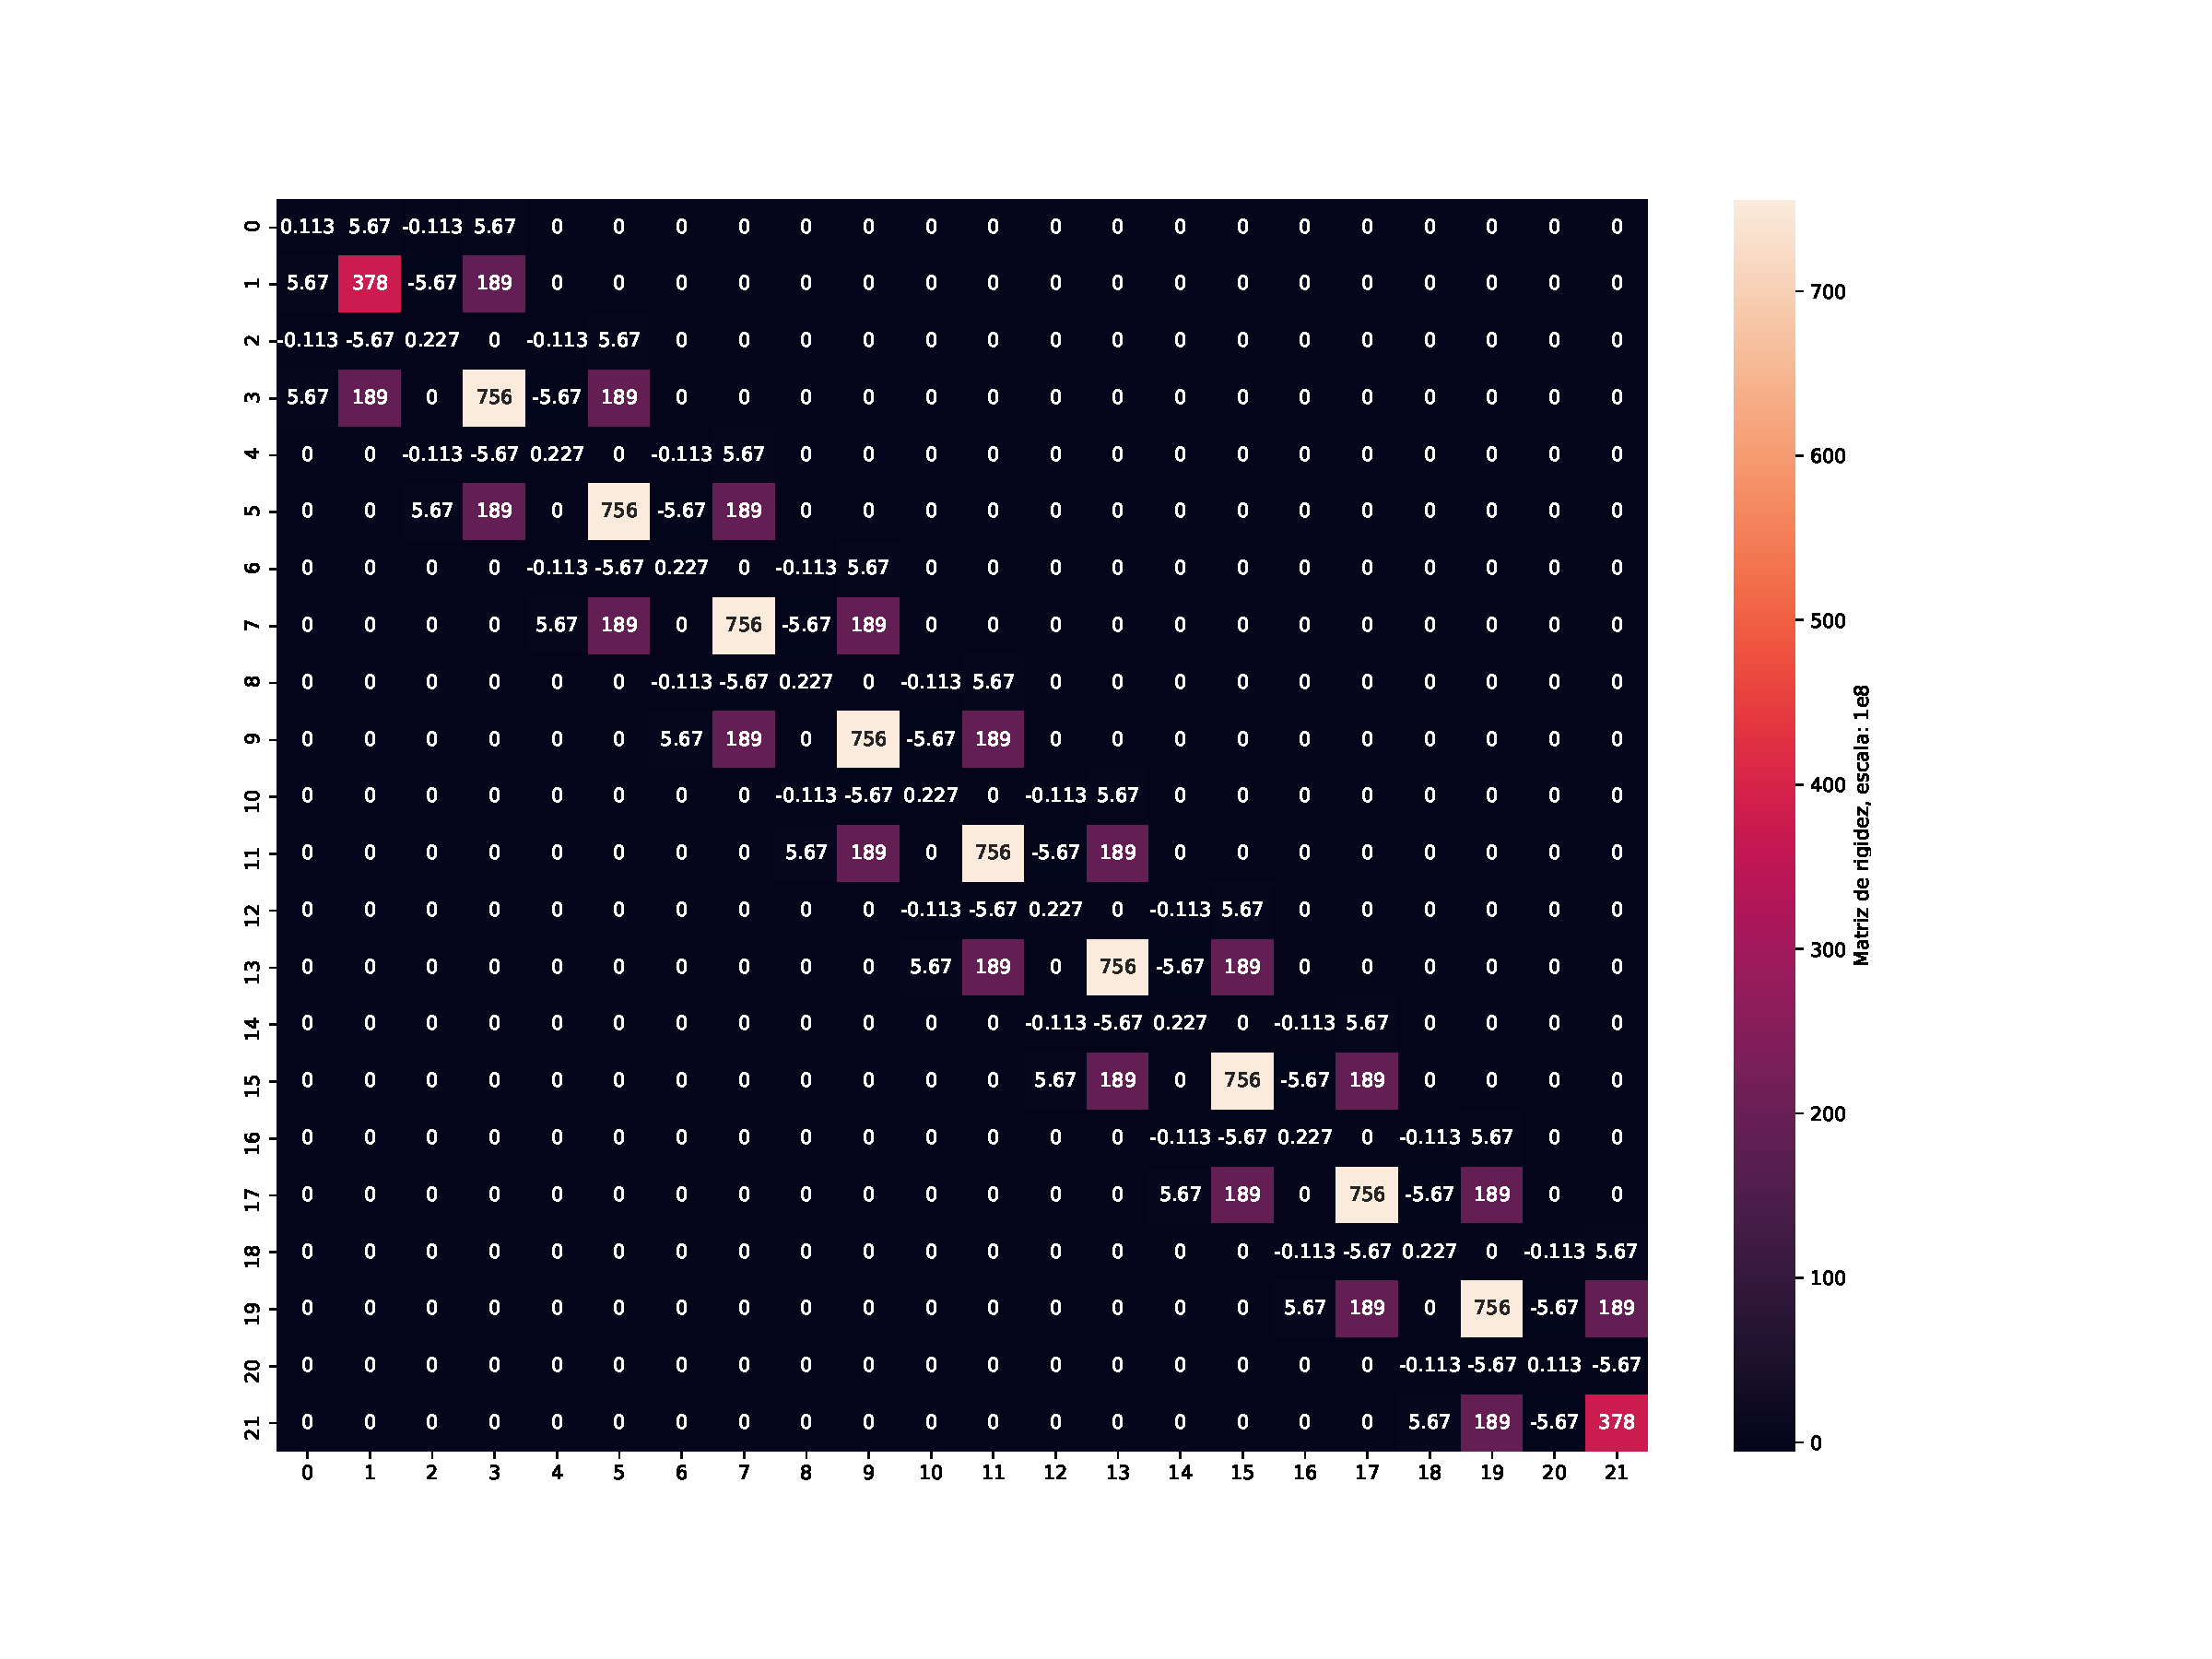
\includegraphics[scale=0.68]{stiffness.pdf}
    \caption{Matriz de rigidez}
\end{figure}
Se observa que la mayor parte de los elementos son iguales a 0 y que la matriz es completamente simétrica. Estas características especiales de la matriz de rigidez nos permiten utilizar el método del gradiente conjugado para acelerar la solución del problema.
\begin{figure}[H]
    \centering
    \includegraphics[scale=0.75]{representation.pdf}
    \caption{Representación esquemática}
\end{figure}
Los nodos se representan en figura de color {\color{red} rojo} y los elementos de color {\color{blue} azul}.
\newpage
Cada desplazamiento y fuerza corresponde a un nodo en una dirección ($x$, $y$ o $\theta$); por lo que al nodo $i$ le corresponde las reacciones $3i$ ($x$), $3i+1$ ($y$) y $3i+2$ ($\theta$). Se organiza los datos del desplazamiento y fuerza en cada dirección en una tabla para cada nodo para tener una mejor compresión de los resultados:
\begin{figure}[H]
    \centering
    \includegraphics[scale=0.78]{forces.pdf}
    \caption{Reacciones en los nodos}
\end{figure}
Los nodos 0 y 21 son los nodos de apoyo, de la Figura 1, notamos que las reacciones son {\large $F_{0} = [13834.3002, 15.9261]$ N, $M_{0} = 16530.4809$ N-m, $F_{21} = [-18834.3002, 9684.0739]$, $M_{21} = -20639,5274$ N-m.}
\newpage
Mientras que la deformada del bastidor sería
\begin{figure}[H]
    \centering
    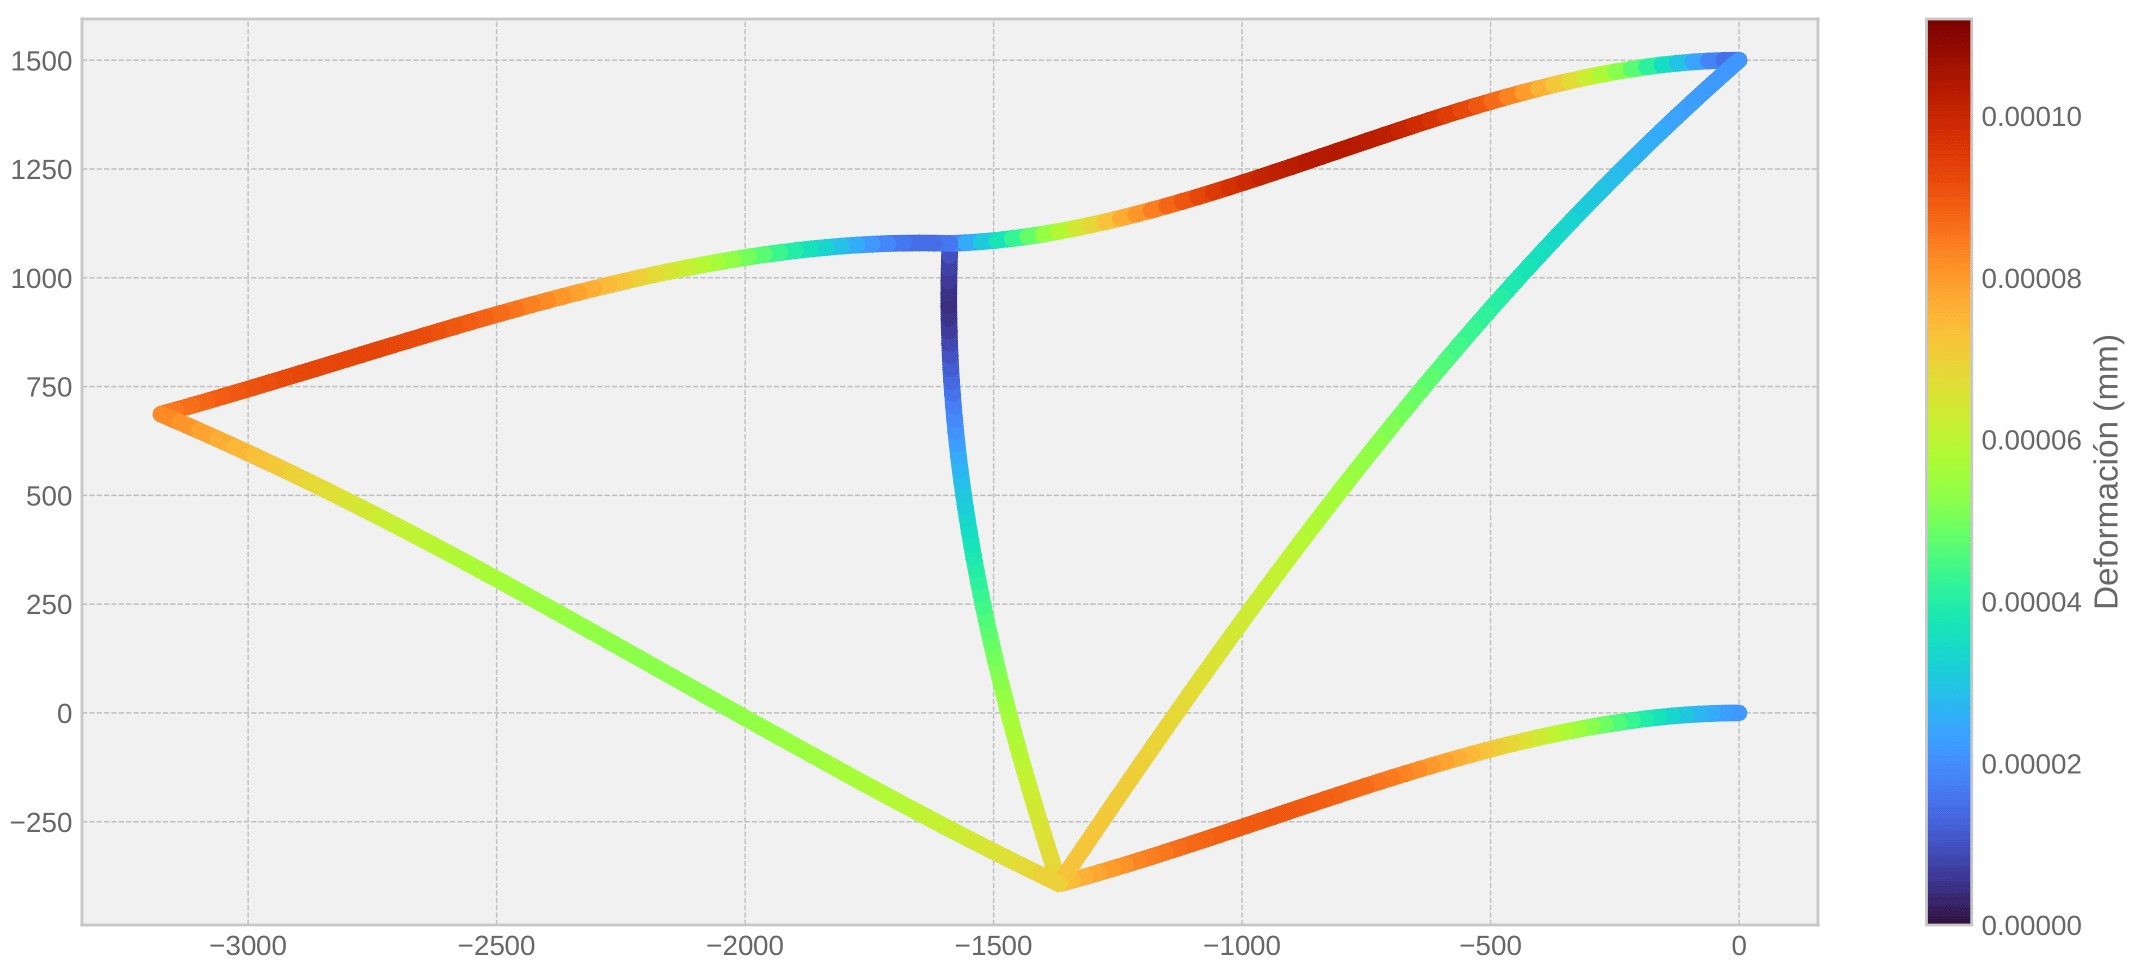
\includegraphics[scale=0.72]{frame.pdf}
    \caption{Deformada del bastidor, escala x4000}
\end{figure}
\begin{figure}[H]
    \centering
    \includegraphics[scale=0.72]{stressM.pdf}
    \caption{Esfuerzo por flexión sobre los elementos con $\xi=-1,0,1$}
\end{figure}
\begin{figure}[H]
    \centering
    \includegraphics[scale=0.72]{stressN.pdf}
    \caption{Esfuerzo por tracción sobre los elementos}
\end{figure}
Organizando las gráficas de esfuerzos en una tabla:
\begin{table}[H]
    \centering
    \tcbox[left=0mm,right=0mm,top=0mm,bottom=0mm,boxsep=0mm,toptitle=0.8mm,bottomtitle=0.8mm,title=Resultados del análisis por elementos finitos]{
    \renewcommand{\arraystretch}{1.3}%
    \begin{tabular}{c|c|c||c|c|c|c}
        \textbf{\footnotesize Elemento} & \textbf{\footnotesize Nodo 1} & \textbf{\footnotesize Nodo 2} & $\sigma_{\mrm{flexion}}$ ($\xi = -1$) MPa & $\sigma_{\mrm{flexion}}$ ($\xi = 0$) MPa & $\sigma_{\mrm{flexion}}$ ($\xi = 1$) MPa & $\sigma_{\mrm{traccion}}$ MPa\\
        \hline
        0 & 0 & 1 & -1.34702 & -1.20798 & -1.06893 & -7.04575 \\
        \hline
        1 & 1 & 2 & -1.06893 & -0.92988 & -0.79084 & -7.04575 \\
        \hline
        2 & 2 & 3 & -0.79084 & -0.65179 & -0.51274 & -7.04575 \\
        \hline
        3 & 3 & 4 & -0.51274 & -0.37369 & -0.23465 & -7.04575 \\
        \hline
        4 & 4 & 5 & -0.23465 & -0.0956 & 0.04345 & -7.04575 \\
        \hline
        5 & 5 & 6 & 0.04345 & 0.1825 & 0.32154 & -7.04575 \\
        \hline
        6 & 6 & 7 & 0.32154 & 0.46059 & 0.59964 & -7.04575 \\
        \hline
        7 & 7 & 8 & 0.21903 & 0.2485 & 0.27797 & -1.51805 \\
        \hline
        8 & 8 & 9 & 0.27797 & 0.30744 & 0.33691 & -1.51805 \\
        \hline
        9 & 9 & 10 & 0.33691 & 0.36638 & 0.39585 & -1.51805 \\
        \hline
        10 & 10 & 11 & 0.39585 & 0.42532 & 0.45479 & -1.51805 \\
        \hline
        11 & 11 & 12 & 0.45479 & 0.48426 & 0.51373 & -1.51805 \\
        \hline
        12 & 12 & 13 & 0.51373 & 0.5432 & 0.57267 & -1.51805 \\
        \hline
        13 & 13 & 14 & 0.57267 & 0.60214 & 0.63161 & -1.51805 \\
        \hline
        14 & 14 & 15 & 2.03972 & 1.74096 & 1.4422 & -4.67924 \\
        \hline
        15 & 15 & 16 & 1.4422 & 1.14343 & 0.84467 & -4.67924 \\
        \hline
        16 & 16 & 17 & 0.84467 & 0.5459 & 0.24714 & -4.67924 \\
        \hline
        17 & 17 & 18 & 0.24714 & -0.05162 & -0.35039 & -4.67924 \\
        \hline
        18 & 18 & 19 & -0.35039 & -0.64915 & -0.94791 & -4.67924 \\
        \hline
        19 & 19 & 20 & -0.94791 & -1.24668 & -1.54544 & -4.67924 \\
        \hline
        20 & 20 & 21 & -1.54544 & -1.84421 & -2.14297 & -4.67924 \\
        \hline
        21 & 21 & 22 & -0.46111 & -0.43299 & -0.40486 & 6.94918 \\
        \hline
        22 & 22 & 23 & -0.40486 & -0.37674 & -0.34861 & 6.94918 \\
        \hline
        23 & 23 & 24 & -0.34861 & -0.32049 & -0.29236 & 6.94918 \\
        \hline
        24 & 24 & 25 & -0.29236 & -0.26424 & -0.23612 & 6.94918 \\
        \hline
        25 & 25 & 26 & -0.23612 & -0.20799 & -0.17987 & 6.94918 \\
        \hline
        26 & 26 & 27 & -0.17987 & -0.15174 & -0.12362 & 6.94918 \\
        \hline
        27 & 27 & 7 & -0.12362 & -0.0955 & -0.06737 & 6.94918 \\
        \hline
        28 & 14 & 28 & -1.40812 & -1.27794 & -1.14776 & 4.68096 \\
        \hline
        29 & 28 & 29 & -1.14776 & -1.01758 & -0.88739 & 4.68096 \\
        \hline
        30 & 29 & 30 & -0.88739 & -0.75721 & -0.62703 & 4.68096 \\
        \hline
        31 & 30 & 31 & -0.62703 & -0.49685 & -0.36667 & 4.68096 \\
        \hline
        32 & 31 & 32 & -0.36667 & -0.23649 & -0.10631 & 4.68096 \\
        \hline
        33 & 32 & 33 & -0.10631 & 0.02387 & 0.15405 & 4.68096 \\
        \hline
        34 & 33 & 34 & 0.15405 & 0.28423 & 0.41441 & 4.68096 \\
        \hline
        35 & 34 & 35 & 0.41441 & 0.36243 & 0.31046 & -3.01647 \\
        \hline
        36 & 35 & 36 & 0.31046 & 0.25848 & 0.20651 & -3.01647 \\
        \hline
        37 & 36 & 37 & 0.20651 & 0.15453 & 0.10256 & -3.01647 \\
        \hline
        38 & 37 & 38 & 0.10256 & 0.05058 & -0.00139 & -3.01647 \\
        \hline
        39 & 38 & 39 & -0.00139 & -0.05337 & -0.10534 & -3.01647 \\
        \hline
        40 & 39 & 40 & -0.10534 & -0.15732 & -0.20929 & -3.01647 \\
        \hline
        41 & 40 & 7 & -0.20929 & -0.26127 & -0.31324 & -3.01647
    \end{tabular}}
    \caption{Esfuerzos en los elementos finitos}
\end{table}
Las gráficas de esfuerzos y deformaciones en el bastidor:
\begin{figure}[H]
    \centering
    \includegraphics[scale=0.725]{frame_stress_M.pdf}
    \caption{Esfuerzo por flexión}
\end{figure}
\begin{figure}[H]
    \centering
    \includegraphics[scale=0.725]{frame_stress_N.pdf}
    \caption{Esfuerzo por tracción}
\end{figure}

\begin{figure}[H]
    \centering
    \includegraphics[scale=0.725]{deformation.pdf}
    \caption{Deformación de los elementos}
\end{figure}

\section{Generalización para $\mathbf{n}$ elementos}
Al incrementar la cantidad de elementos se obtiene mayor información sobre los esfuerzos por flexión en el bastidor y su deformada. Por ejemplo para 1000 elementos en el bastidor, obtenemos la siguiente deformada:
\begin{figure}[H]
    \centering
    \includegraphics[scale=0.68]{real_displacement.pdf}
    \caption{Deformada del bastidor, escala x4000}
\end{figure}
Mientras que el mapa de calor de la deformación de los elementos sería:
\begin{figure}[H]
    \centering
    \includegraphics[scale=0.68]{real_deformation.pdf}
    \caption{Mapa de calor de la deformación de los elementos}
\end{figure}
Observamos que la mayor deformación del bastidor ocurre en la parte superior derecha. Esto debido principalmente a la flexión que ocasionan las cargas, esto se detalla en los gráficos de esfuerzo del bastidor:
\begin{figure}[H]
    \centering
    \includegraphics[scale=0.68]{real_stress_M.pdf}
    \caption{Esfuerzo por flexión}
\end{figure}
Observamos que efectivamente, el esfuerzo por flexión es mayor en los elementos situados en la parte superior derecha. Teniendo la variación más grande de esfuerzo por flexión en comparación con los demás elementos. Mientras que en la gráfica de esfuerzo por tracción, son todos los elementos de la parte derecha que tienen un esfuerzo igual a $\pm 6$ MPa.
\begin{figure}[H]
    \centering
    \includegraphics[scale=0.68]{real_stress_N.pdf}
    \caption{Esfuerzo por tracción}
\end{figure}
\newpage
\section{Verificación de resultados en Autodesk Fusion 360}
Se modela el bastidor en Autodesk Fusion 360
\begin{figure}[H]
    \centering
    \includegraphics[scale=0.5]{render.png}
    \caption{Renderizado de la geometría del bastidor}
\end{figure}
Posteriormente se simula el bastidor junto a las cargas y el material del problema, y se obtienen los resultados para el esfuerzo.
\begin{figure}[H]
    \centering
    \includegraphics[scale=0.55]{xd.png}
    \caption{Deformación y flecha máxima de la viga a 493 mm}
\end{figure}
Observamos que los esfuerzos sobre los elementos del bastidor corresponden a los obtenidos por el código realizado.
\newpage
\section*{Conclusiones}
\begin{enumerate}
    \item De la tabla de reacciones en los nodos, observamos que dichas reacciones se encuentran en los apoyos, dando como valores $F_{0} = [13834.3002, 15.9261]$ N, $M_{0} = 16530.4809$ N-m, $F_{21} = [-18834.3002, 9684.0739]$, $M_{21} = -20639,5274$ N-m.
    \item Observamos en la gráfica de esfuerzos por flexión que los valores obtenidos según $\xi$ son muy cercanos, esto es debido a la condición de continuidad del esfuerzo en un elemento finito. Si se aumentará la cantidad de nodos por elemento del bastidor ($n$) estos esfuerzos deben converger a un único valor para todo $-1 \geq \xi \leq 1$.
    \item Los resultados obtenidos por el código realizado y la simulación hecha en Autodesk Fusion 360 nos dan resultados similares.
    \item Los esfuerzos por tracción, se esperaba que se mantuviesen constante para cada elemento del bastidor, tal como se muestra en la gráfica obtenida.
    \item Es necesario añadir por lo menos un nodo en cada elemento del bastidor para apreciar como se deforma por la flexión.
    \item El parámetro $n$ del código indica la cantidad de nodos a utilizar por cada elemento del bastidor. Esto nos permite poder modificar la cantidad total de elementos y la precisión de los resultados de forma rápida. 
\end{enumerate}
\begin{thebibliography}{9}
\bibitem{d1} Optimized methods in FEM:\\
https://www.sciencedirect.com/topics/engineering/gauss-seidel-method
\bibitem{d3}
Sparse Matrix:\\
https://en.wikipedia.org/wiki/Sparse$\_$matrix
\bibitem{d4}
Sparse Matrix Library:\\
https://github.com/uestla/Sparse-Matrix
\bibitem{d5}
Mailman algorithm:\\
http://www.cs.yale.edu/homes/el327/papers/matrixVectorApp.pdf
\bibitem{d6}
Fast Algorithms with Preprocessing for Matrix-Vector Multiplication Problems:\\
https://www.sciencedirect.com/science/article/pii/S0885064X84710211
\end{thebibliography}
%\bibliographystyle{IEEEtran}
%\bibliography{IEEEabrv,sample}

%\animategraphics[height=3.4in,autoplay,controls]{4}{frame}{0}{23}
\end{document}
